% article example for classicthesis.sty
\documentclass[10pt,a4paper]{article} % KOMA-Script article scrartcl
\usepackage{import}
\usepackage{xifthen}
\usepackage{pdfpages}
\usepackage{transparent}
\newcommand{\incfig}[1]{%
    \def\svgwidth{\columnwidth}
    \import{./figures/}{#1.pdf_tex}
}
\usepackage{lipsum}     %lorem ipsum text
\usepackage{titlesec}   %Section settings
\usepackage{titling}    %Title settings
\usepackage[margin=10em]{geometry}  %Adjusting margins
\usepackage{setspace}
\usepackage{listings}
\usepackage{amsmath}    %Display equations options
\usepackage{amssymb}    %More symbols
\usepackage{xcolor}     %Color settings
\usepackage{pagecolor}
\usepackage{mdframed}
\usepackage[utf8]{inputenc}
\usepackage{longtable}
\usepackage{multicol}
\usepackage{graphicx}
\graphicspath{ {./Images/} }
\setlength{\columnsep}{1cm}

% ====| color de la pagina y del fondo |==== %
\pagecolor{black}
\color{white}



\begin{document}
    %========================{TITLE}====================%
    \title{{  13th lab of Forensics  }}
    \author{{Rodrigo Castillo}}
    \date{\today}

    \maketitle


     % ====| Loguito |==== %
    
\includegraphics[width=0.1\linewidth]{negro_cara.png}
    %=======================NOTES GOES HERE===================%

    \section{Read the section "Recopilación de evidencias" at page 19, and
    explain in your own words the order in which evidences must be gathered}

    the idea beside gathering evidences is to take a state of the system as
    close as can be possible, however, there are information that is more
    volatile than other, so the idea of gathering evidence is to prioritize the
    gathering of information that is more volatile before information that is
    not and can be gaterher later.
    \\
    the information that must be gathered  is ...
    \begin{enumerate}
        \item {content in the memory}
        \item {connection state}
        \item {state of process of execution}
        \item {content inside the hard disks}
        \item {content in hard drives}
    \end{enumerate}
    inside of volatile evidence , is important to check as fast as possible
    is...
    \begin{enumerate}
        \item {date}
        \item {processes that are running on the machine (top)}
        \item {network processes}
        \item {prots openned (TCP/UDP)}
        \item {users connected remotely}
    \end{enumerate}

    \newpage
    \section{captures}
    for the following task, i'll make one script that will execute all the
    commands listed on the table and then i'll explain every command on the
    table.
    The script...
    \begin{figure}[h!]
        \centering
        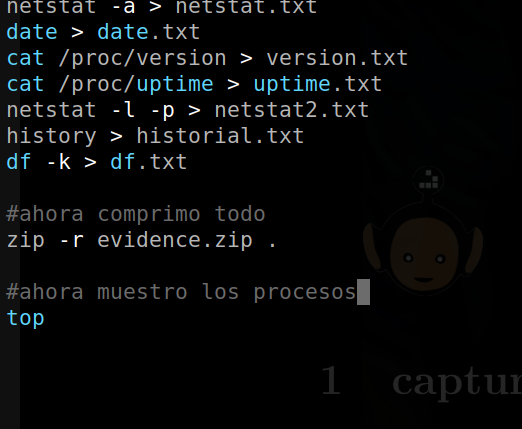
\includegraphics[width=0.5\linewidth]{script.png}
        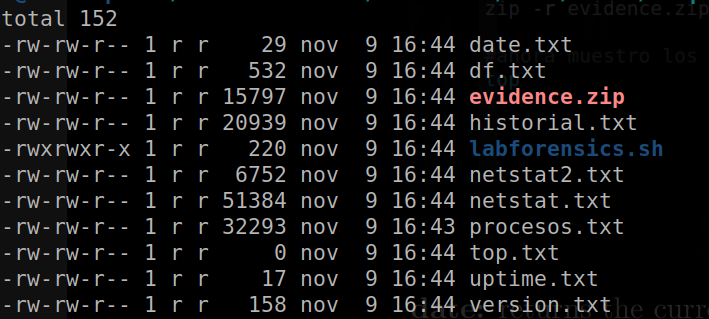
\includegraphics[width=0.5\linewidth]{result.png}
        \caption{script and result}
        \label{script}
    \end{figure}

    \textbf{date:} returns the current date .
    \\
    \textbf{df:} returns the current state of the disks .
    \\
    \textbf{history:} return the history of bash commands .
    \\
    \textbf{netstat:} return the current state of wireless conections.
    \\
    \textbf{top:} return the current processes running.
    \\
    \textbf{uptime}  return the cuantity of time that the machine has been on.
    \\
    \textbf{version} return the linux version.

    \newpage
    \section{Practical part}

    \begin{figure}[h!]
        \centering
        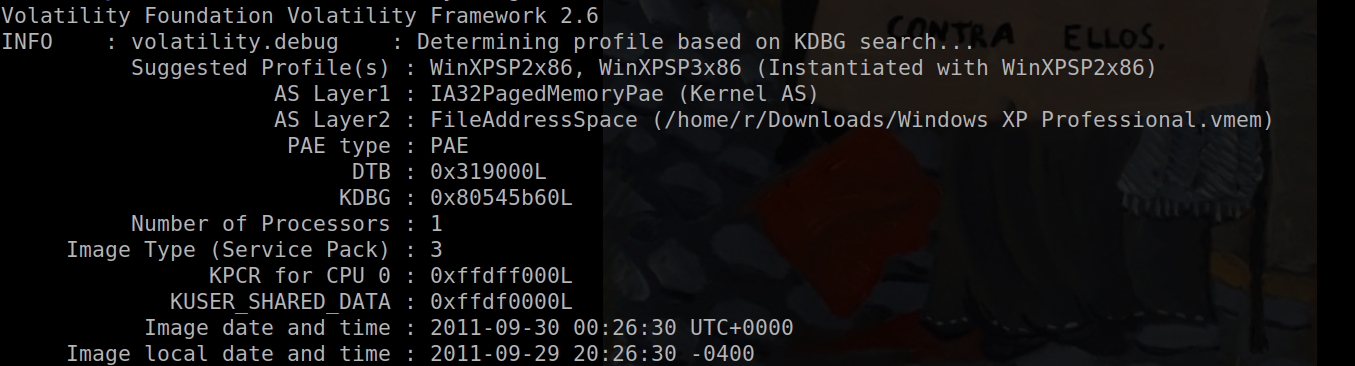
\includegraphics[width=0.8\linewidth]{imageinfo.png}
        \caption{image info}
        \label{volatility1}
    \end{figure}

    \begin{figure}[h!]
        \centering
        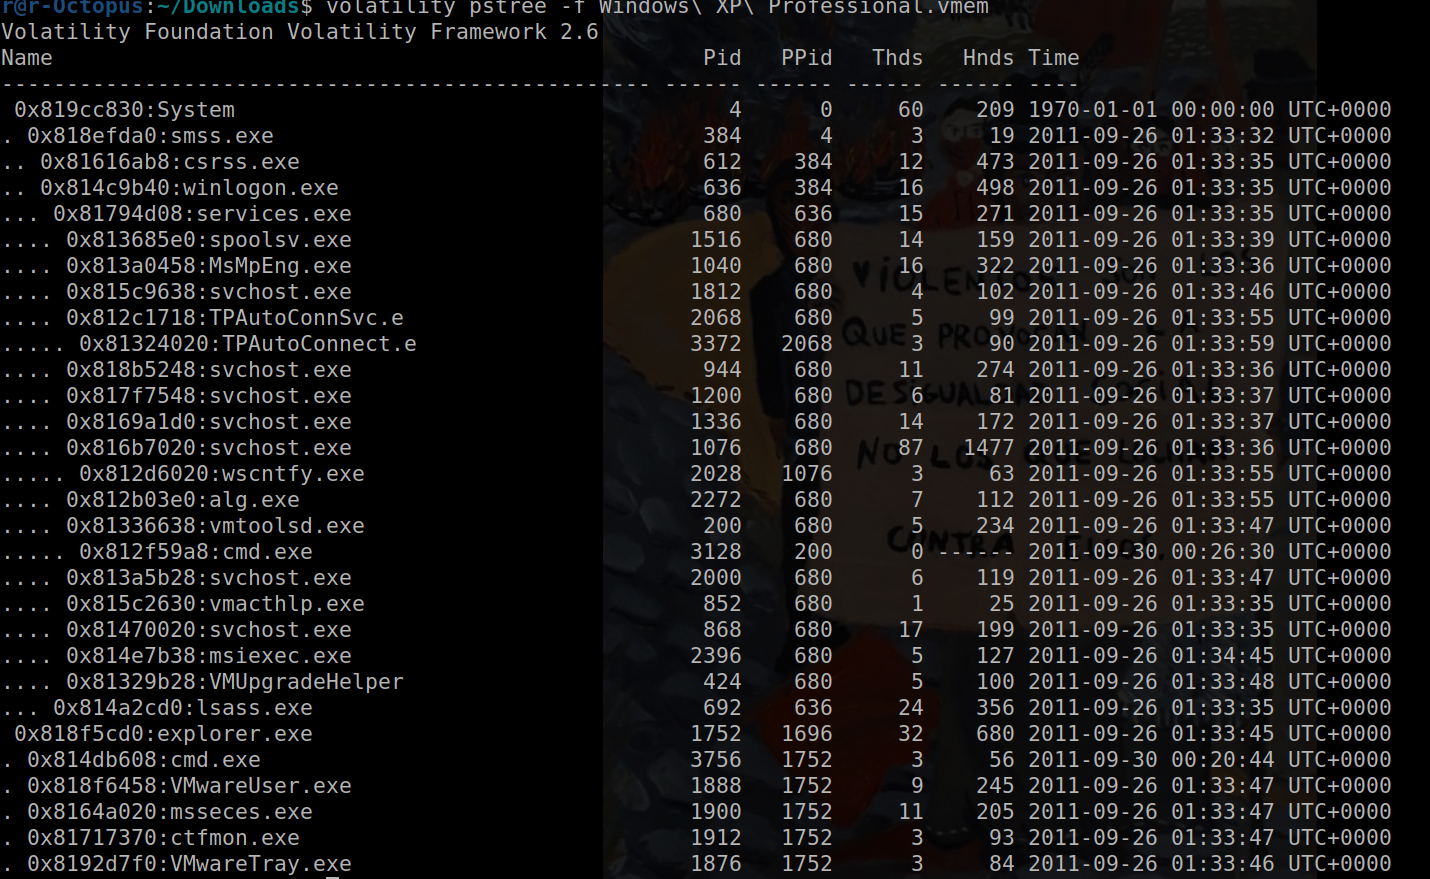
\includegraphics[width=1\linewidth]{pstree.png}
        \caption{pstree}
        \label{fig}
    \end{figure}

    \begin{figure}[h!]
        \centering
        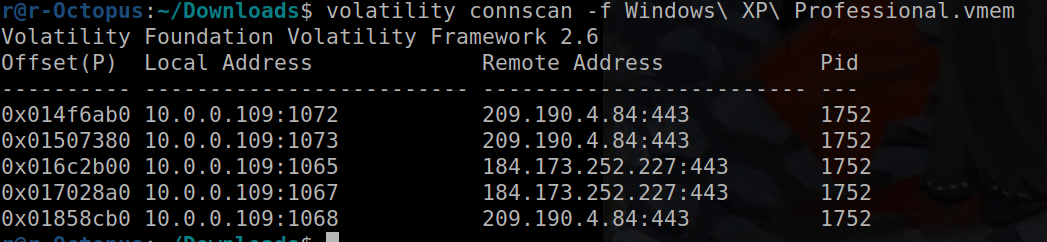
\includegraphics[width=0.8\linewidth]{connscan.png}
        \caption{connscan}
        \label{fig}
    \end{figure}

    \begin{figure}[h!]
        \centering
        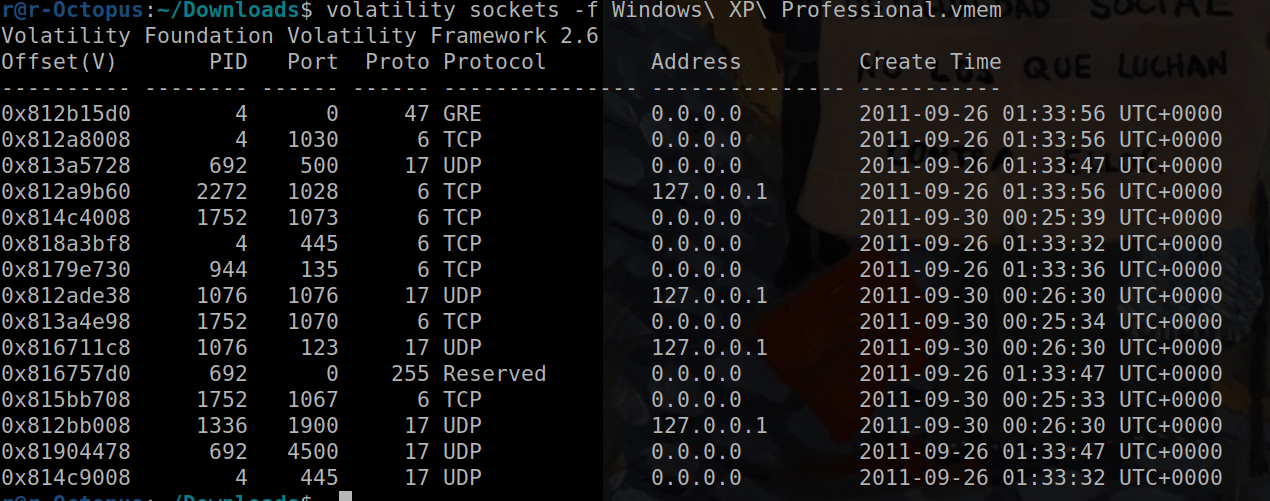
\includegraphics[width=0.8\linewidth]{sockets.png}
        \caption{sockets}
        \label{fig}
    \end{figure}

    \begin{figure}[h!]
        \centering
        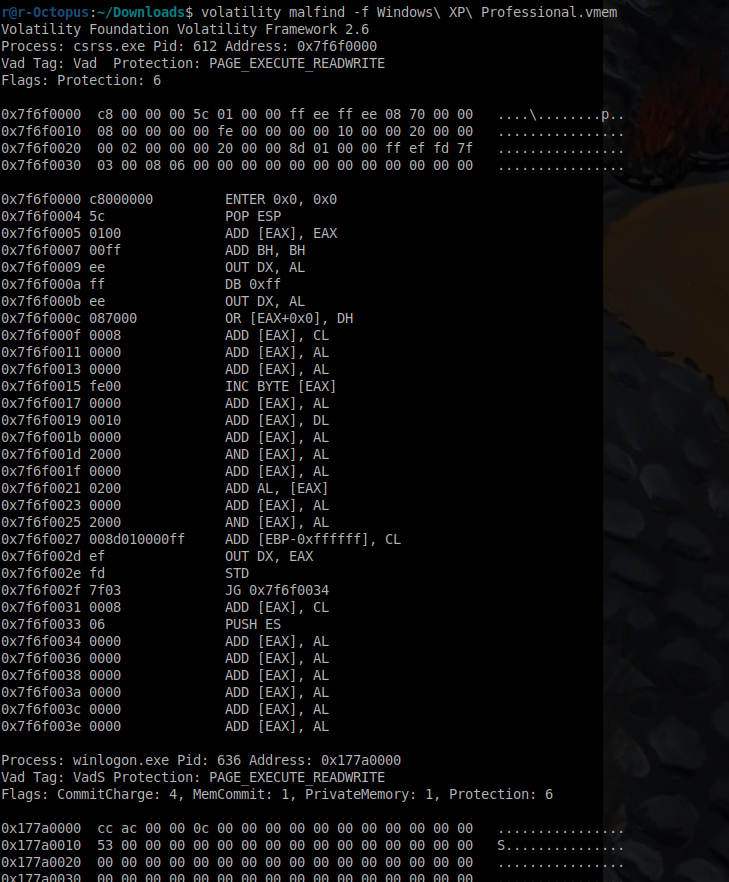
\includegraphics[width=0.8\linewidth]{malfind.png}
        \caption{nombre}
        \label{fig}
    \end{figure}

    \begin{figure}[h!]
        \centering
        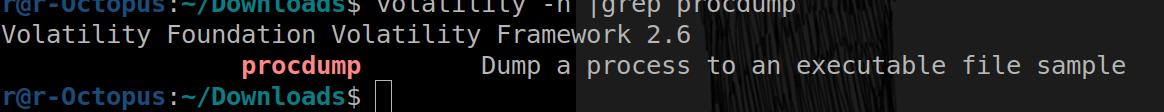
\includegraphics[width=0.8\linewidth]{procdumpin.png}
        \caption{manual of the prodcump flag}
        \label{fig}
    \end{figure}


















    %=======================NOTES ENDS HERE===================%

    % bib stuff
    \nocite{*}
    \addtocontents{toc}{{}}
    \addcontentsline{toc}{section}{\refname}
    \bibliographystyle{plain}
    \bibliography{../Bibliography}
\end{document}
